\chapter{The Fibonacci Sequence — Nature’s Algorithm}

\section{The Story of Fibonacci}
Long ago, in a quiet Italian village, a mathematician named Leonardo of Pisa—nicknamed \textbf{Fibonacci}—noticed patterns in nature that seemed to whisper numbers into every petal, every pinecone, every spiral galaxy.

The Fibonacci sequence begins simply:
\[
F(0) = 0, \quad F(1) = 1,
\]
and each term afterwards is born from the sum of its two predecessors:
\[
F(n) = F(n-1) + F(n-2).
\]
So, the sequence grows:
\[
0, \; 1, \; 1, \; 2, \; 3, \; 5, \; 8, \; 13, \; 21, \; 34, \ldots
\]

Each generation in this sequence depends upon the previous two—just as branches split from branches, and ideas sprout from ideas.

\vspace{1em}
\begin{center}
\textit{Recursion is nature’s favorite loop.}
\end{center}
\vspace{1em}

\section{Seeing the Pattern}
To visualize how recursion unfolds, consider the computation of $F(5)$:

\[
\texttt{fib(5)} \rightarrow \texttt{fib(4)} + \texttt{fib(3)}
\]

Each call branches into two smaller ones, creating a beautiful tree of self-reference:

\begin{center}
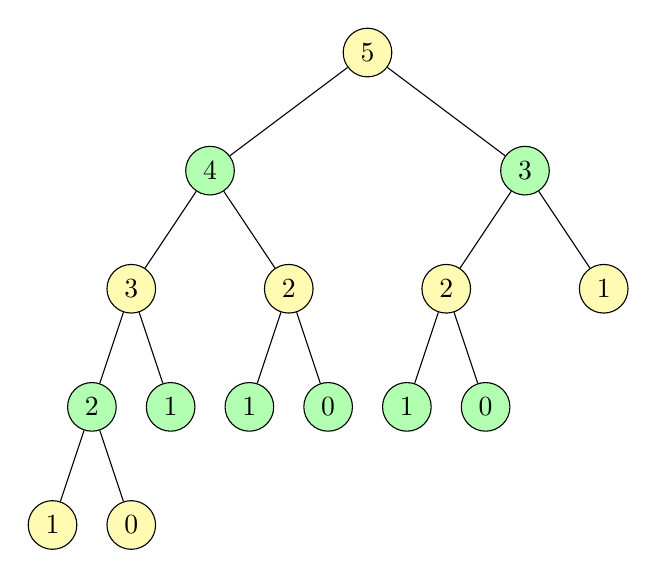
\begin{tikzpicture}[level distance=1.5cm,
  level 1/.style={sibling distance=4cm},
  level 2/.style={sibling distance=2cm},
  level 3/.style={sibling distance=1cm}]
  \node[circle,draw,fill=yellow!30]{5}
    child {node[circle,draw,fill=green!30]{4}
      child {node[circle,draw,fill=yellow!30]{3}
        child {node[circle,draw,fill=green!30]{2}
          child {node[circle,draw,fill=yellow!30]{1}}
          child {node[circle,draw,fill=yellow!30]{0}}}
        child {node[circle,draw,fill=green!30]{1}}}
      child {node[circle,draw,fill=yellow!30]{2}
        child {node[circle,draw,fill=green!30]{1}}
        child {node[circle,draw,fill=green!30]{0}}}}
    child {node[circle,draw,fill=green!30]{3}
      child {node[circle,draw,fill=yellow!30]{2}
        child {node[circle,draw,fill=green!30]{1}}
        child {node[circle,draw,fill=green!30]{0}}}
      child {node[circle,draw,fill=yellow!30]{1}}};
\end{tikzpicture}
\end{center}

Notice how each recursive call duplicates work from previous branches.  
This inefficiency is the price of elegance—but later, we’ll learn to make it faster.

\section{A Gentle Python Introduction}

\begin{verbatim}
def fib_recursive(n):
    """Return the nth Fibonacci number using recursion."""
    if n <= 1:
        return n
    return fib_recursive(n - 1) + fib_recursive(n - 2)

for i in range(10):
    print(f"F({i}) = {fib_recursive(i)}")
\end{verbatim}

Let’s unpack what happens.  
When you call \texttt{fib\_recursive(5)}, the function calls itself twice,  
then each of those calls calls itself twice more,  
until it reaches the \textbf{base cases} where $n = 0$ or $n = 1$.

Each branch blooms, divides, and resolves—just like the petals of a sunflower spiraling toward the sun.

\section{Recursive Beauty}
Recursion is powerful because it mirrors the way we define patterns in nature:  
each step depends upon smaller, simpler versions of itself.

\begin{quote}
\textit{To understand recursion, one must first understand recursion.}
\end{quote}

This idea is both a mathematical truth and a philosophical koan.  
In the next chapters, we’ll measure just how costly this beauty is,  
and how algorithmic growth behaves as $n$ increases.

\begin{center}
\textbf{Coming soon:}\\
\textit{Chapter 4 — Measuring the Cost of Recursion}\\
\textit{and}\\
\textit{Chapter 5 — Understanding Big-O Through Fibonacci.}
\end{center}

